\section{Teorema de Arnold-Liouville}\label{sec:arnoldliouville}
A la hora de estudiar sistemas dinámicos, una cuestión interesante a plantearse, con consecuencias prácticas y también de carácter fundamental, es si las ecuaciones del sistema podrán ser «integradas», es decir, si podrán ser resueltas mediante integrales («cuadraturas») de funciones conocidas. Decimos entonces que una ecuación diferencial es \emph{integrable por cuadraturas} si es posible escribir su solución general en términos de sumas, productos, composiciones e integrales de funciones conocidas. 

En 1885, Joseph Liouville encontró una condición necesaria para que las ecuaciones de Hamilton de ciertos sistemas hamiltonianos fueran (localmente) integrables por cuadraturas. Décadas más tarde, con la introducción del formalismo geométrico y topológico al estudio de los sistemas dinámicos se descubrirían muchas más cosas interesantes sobre los sistemas que cumplían la condición que Liouville propuso. Destaca especialmente en todo este estudio la teoría de los toros invariantes desarrollada por Vladimir Arnold en 1963. Nace así la teoría de los \emph{sistemas integrables}, cuyos resultados más básicos constituyen el \emph{teorema de Arnold-Liouville}.

\begin{defn}
  \em
  Sea $(M,H)$ un sistema hamiltoniano con $\dim(M)=2n$. Decimos que $(M,H)$ es \emph{integrable (en el sentido de Liouville)} si existen $F_1(=H),\dots,F_n\in \mathscr{C}^{\infty}(M)$ tales que
\begin{enumerate}
  \item son \emph{funcionalmente independientes}, es decir, $\dd F_{1,x}\wedge \dots \wedge \dd F_{n,x}\neq 0$ para casi todo punto\footnote{Como aquí en principio no estamos considerando ninguna medida, con \emph{para casi todo punto} queremos decir en un conjunto \emph{residual} o \emph{comagro}, esto es, que su complementario sea \emph{magro}. Un conjunto se dice \emph{magro} o \emph{de primera categoría de Baire} si es unión numerable de conjuntos diseminados, esto es, de conjuntos cuya adherencia tiene interior vacío. Por ejemplo, el conjunto de los números racionales $\mathbb{Q}\subset\RR$ no es diseminado pero sí es magro en $\RR$. }, 
  \item están \emph{en involución}, esto es, $\pois{F_i}{F_j}=0$ para cada $i,j=1,\dots,n$, y
  \item  los campos $X^{F_i}$ son completos para cada $i=1,\dots,n$. 
\end{enumerate}
Nótese que, como $F_1=H$, en particular, todas las funciones $F_1,\dots,F_n$ son integrales primeras del sistema.

Si escribimos $F:M\rightarrow \RR^n$ con $F(x)=(F_1(x),\dots,F_n(x))$. Los puntos $x\in M$ en los que $\mathrm{rango} (\dd F_x) =n$ se dicen \emph{puntos regulares} del sistema. Los puntos que no son regulares se dicen \emph{puntos críticos}. Si $x\in M$ es un punto crítico, $F(x)$ se dice un \emph{valor crítico}. Si $\Sigma$ es el conjunto de los puntos críticos, $F(\Sigma)\in \RR^n$ se llama \emph{diagrama de bifurcación} del sistema.
 Nótese que, por el teorema de Sard, el diagrama de bifurcación tiene medida nula.
\end{defn}

\begin{obs}
  \em
  De la definición y de la conservación de la energía directamente se deduce que todo sistema con un grado de libertad (y cuyo hamiltoniano sea regular en casi todo punto) es integrable en el sentido de Liouville. Asimismo, un sistema con dos grados de libertad que tenga una cantidad conservada a parte de la energía también será integrable en el sentido de Liouville, ya que las cantidades conservadas dan 0 al evaluar el corchete de Poisson de ellas con el hamiltoniano.
\end{obs}

\begin{thm}[Arnold-Liouville]\label{arnold}
Sea $(M,H)$ un sistema integrable en el sentido de Liouville con $F_1,\dots,F_n$ las funciones en involución.

   Sea $x\in M$ un punto regular del sistema y sea $a=F(x)$. Sea $M_a$ la componente conexa del conjunto de nivel $F^{-1}(a)$ que contiene a $x$. Supongamos además que todo punto de $M_a$ es regular. Entonces $M_a$ es una variedad diferenciable invariante bajo el flujo del sistema y $\left. \omega \right|_{M_a}=0$.
  
 Además $M_a$ es difeomorfa a $\TT^k\times \RR^{n-k}$, para cierto $0 \leq k \leq n$. En particular, si $M_a$ es compacta, $M_a$ es difeomorfa al toro $n$-dimensional $\TT^n$. En este caso, se dice que $M_a$ es un \emph{toro de Liouville}. 
 
 Podemos tomar unas coordenadas $w=(w_1,\dots w_n)$ en $M_a$ de manera que existen unas velocidades constantes $v(a)=(v_1(a),\dots,v_n(a))$ tales que $\dot w (t)=v$. Como consecuencia, las ecuaciones de Hamilton del sistema son localmente integrables por cuadraturas en un entorno de $x$.

\end{thm}

 \begin{proof}
  En primer lugar, como $F$ tiene rango máximo en cada punto de $M_a$, por el teorema de la función implícita $M_a$ es una subvariedad regular de $M$ de dimensión $2n-n=n$. 
  Como $M$ es una variedad simpléctica, para cada $i=1,\dots,n$, podemos definir el campo $X_i=X^{F_i}$. Al ser las $\dd F_i$ linealmente independientes los campos $X_i$ son linealmente independientes. Además, por el teorema de Noether, como para cada $i,j= 1,\dots,n$ $\pois{F_i}{F_j}=0$ (luego es constante), entonces $\lie{X_i}{X_j}=0$. Por esto mismo, la derivada de la función $F_i$ en la dirección de $X_j$ es 0, luego los campos $X_j$ son tangentes a $M_a$.

  De aquí sacamos varias conclusiones:
  \begin{enumerate}
    \item $M_a$ es invariante con respecto a cada uno de los $n$ flujos hamiltonianos generados por cada función $F_i$ (luego, en particular lo será respecto del generado por $F_1$).
    \item Como, para cada $x \in M_a$, los campos $X_1|_x,\dots, X_n|_x$ forman una base de $T_x M_a$, sean $X_x, Y_x \in T_x M_a$, entonces $X_x = \sum_{i=1}^n b_i X_i|_x$, $Y_x=\sum_{i=1}^n c_i X_i|_x$. Ahora,
      \[
	\omega(X_x,Y_x)= \sum_{i,j=1}^n b_i c_j \omega(X_i|_x,X_j|_x) = \sum_{i,j=1}^n b_i c_j \{F_j,F_i\} = 0.
      \]
      Por tanto, $\omega$ se anula en $T_x M_a$. 
    \item $M_a$ es una variedad diferenciable de dimensión $n$ con $n$ campos conmutativos dos a dos y linealmente independientes en todo punto de $M_a$. 
  \end{enumerate}

  Esto prueba la primera parte del teorema. Para continuar, necesitamos probar un lema previo.

  \begin{lema}\label{lemtoro}
    Sea $M$ una variedad diferenciable de dimensión $n$ conexa y compacta tal que existen campos $X_1,\dots,X_n$ en $M$ completos y linealmente independientes y tales que, para todo $i,j=1,\dots,n$, $i\neq j$, $[X_i,X_j]=0$. Entonces $M$ es difeomorfa a $\TT^k\times \RR^{n-k}$. 
\end{lema}
\begin{proof}(del Lema \ref{lemtoro}).
  Para cada $i=1,\dots,n$, sea $g_i$ el flujo completo generado por $X_i$. Como para todo $i\neq j$ $[X_i,X_j]=0 $ entonces $g_i$ conmuta con $g_j$, es decir, $g_ig_j (x)=g_jg_i (x)$, para todo $x \in M$. 

  Así, podemos definir una acción de $\RR^n$ en $M$ que a cada $t=(t_1,\dots,t_n)\in \RR^n$ le asigna $g_t:M\rightarrow M,$ con $g_t=g_{1,t_1}\cdots g_{n,t_n}$.
Por conmutar los flujos, $g_{t+s}=g_t g_s$. Ahora, fijo $x_0 \in M$, definimos 
\[
  \begin{array}{rcl}
g:\RR^n & \longrightarrow & M \\
t & \longmapsto & g_t (x_0).
\end{array}
\]

Como los campos son linealmente independientes, $d_t g$ es un isomorfismo lineal para todo $t$ y, por el teorema de la función implícita, $g$ es un difeomorfismo local. Además, sea $x\in M$, tomamos una curva $\gamma$ que una $x$ y $x_0$ y una sucesión finita de entornos $V_1,\dots,V_n$ que recubran $\gamma$, en los que $g$ sea difeomorfismo y tales que $x_0 \in V_1$, $x \in V_n$. Para cada $i=1,\dots,n-1$, sea $x_i \in V_i \cap V_{i+1}$ y sea $x_n=x$. Para cada $i=0,\dots,n-1$, centramos $g$ en $x_i$ (de tal forma que $g(0)=x_i$) en el entorno $V_{i+1}$ y lo llamamos $g_i$. Definimos $t_i$ tal que $g_{i-1,t_i}(x_{i-1})=x_i$, entonces,
\[
  x=g_{n-1,t_n}(x_{n-1})=g_{n-1,t_n}g_{n-2,t_{n-1}}(x_{n-2})=\cdots=g_{n-1,t_{n}}\cdots g_{0,t_1} (x_0),
\]
luego, sea $t=t_1+\cdots+t_n$, $x=g_t (x_0)$. Por tanto, $g$ es sobreyectiva.
\begin{figure}[h]
  \centering
  \includegraphics[width=0.5\textwidth]{pics/entornos.eps}
  \caption{\small Idea de la demostración de que $g$ es sobreyectiva.}
  \label{fig:entornos}
\end{figure}

Tenemos entonces que $g:\RR^n\rightarrow M$ es un difeomorfismo local sobreyectivo, luego es una identificación diferenciable, de modo que si llamamos 
\[  
  H:=\{t \in \RR^n \mid g_t(x_0)=x_0\},
\]
entonces, por la propiedad universal del cociente, el siguiente diagrama
\begin{center}
  \begin{tikzcd}
    \RR^n \arrow{r}{g}\arrow{d}{} & M    \\ 
    \RR^n/H, \arrow{ru}{}
  \end{tikzcd}
\end{center}
da un difeomorfismo entre $M$ y $\RR^n/H$. Si $H$ es vacío, $M\cong \RR^n$ y habríamos terminado. Supongamos que $H$ es no vacío.
 Entonces, dados $t, s \in H$, 
\[
  g_{s+t}(x_0)=g_sg_t(x_0)=g_s(x_0)=x_0
\]
y 
\[
  g_{-t}(x_0)=g_{-t}g_t(x_0)=x_0.
\] 
Es decir, $H$ es un subgrupo de $(\RR^n,+)$. Además, $H$ no depende de la elección de $x_0$, en efecto, si $x=g_r (x_0)$ y $t\in H$, entonces 
\[
  g_t (x) = g_{t+r}(x_0)=g_rg_t(x_0)=g_r(x_0)=x. 
 \] 

 Como $g$ es un difeomorfismo local, existe un entorno $V\subset \RR^n$ de 0 tal que $H\cap V= \{0\}$. Es más, sean $t\in H$, $s\in V\backslash \{0\}$ y $x\in M$, 
  \[
    g_{t+s}(x)=g_sg_t(x)=g_s(x)\neq x.
  \]
  Luego $H$ es un conjunto discreto. 
  \begin{figure}[h]
    \centering
    \includegraphics[width=0.2\textwidth]{pics/discreto}
    \caption{\small Idea de que $H$ es discreto.}
    \label{fig:discreto}
  \end{figure}

  Antes de continuar, es necesario probar el siguiente lema:

  \begin{lema}\label{discreto}
    Todo subgrupo no trivial, cerrado y discreto $H$ de $\RR^n$ es isomorfo a $\ZZ^k$ para algún $k\in\{1,\dots,n\}$. Es decir, existen $e_1,\dots,e_k \in H$ linealmente independientes tales que 
    \[
      H=\{n_1e_1+\cdots+n_ke_k \mid (n_1,\dots,n_k) \in \ZZ^k \}.
    \]
  \end{lema}
  \begin{proof}(del Lema \ref{discreto}). 
  Sea $e_0 \in H$, $e_0 \neq 0$. Como $H$ es discreto, $H \cap B(0,\norm{e_0})$ es finito. De estos puntos, consideramos aquellos que están en $L(e_0)$ \footnote{Aquí $L(x)$ denota la envoltura lineal de $x$.} y de estos escogemos el más cercano, que llamaremos $e_1$. 
  
  Si existieran algún $e \in H$ y algún $m \in \ZZ$ tal que $e \in (me_1,(m+1)e_1)$, entonces $e-me_1 \in H \cap L(e_0)$ estaría más cerca de 0 que $e_1$. Por tanto, 
  \[
    H\cap L(e_0) = e_1\ZZ.
  \]

  Si no hay puntos de $H$ fuera de $L(e_1)$ hemos terminado, $H$ es isomorfo a $\ZZ$. En caso contrario, sea $e \in H \backslash L(e_1)$, proyectamos ortogonalmente $e$ sobre $L(e_1)$. Esta proyección cae exactamente sobre un intervalo $\Delta=[me_1,(m+1)e_1)$ para cierto $m \in \ZZ$. Sea $C$ el cilindro de eje $\Delta$ y de radio igual a la distancia entre $\Delta$ y $e$. $C\cap H$ es finito. De estos puntos, sea $e_2$ el más cercano a $\Delta$ que no esté en $\Delta$. Entonces, para cualquier otro $f \in H$, la distancia entre $f$ y $L(e_1)$ es mayor que la distancia entre $e_2$ y $L(e_1)$. 
    
    En efecto, en tal caso, sea $l \in \ZZ$ tal que la proyección ortogonal de $f$ cae sobre $[le_1,(l+1)e_1)$, entonces $f'=f-le_1+me_1 \in C$ y la distancia entre $f'$ y $L(e_1)$ es menor que la distancia entre $e_2$ y $L(e_1)$, lo que nos lleva a una contradicción.

  \begin{figure}[h]
    \centering
    \includegraphics{pics/grupo}
    \caption{\small Idea de la demostración del lema.}
    \label{fig:grupo}
  \end{figure}

      Ahora, $\{n_1e_1+n_2e_2 \mid (n_1,n_2) \in \ZZ^2 \}$ forma una red discreta en $L(e_1,e_2)$. Además, si existiera un $e\in H$ que no perteneciese a la red, sean $m_1=[\esc{e}{e_1}]$, $m_2=[\esc{e}{e_2}]$. Entonces, $e-m_1e_1-m_2e_2$ estaría más cerca de $L(e_1)$ que $e_2$. Por tanto, esta red es exactamente $L(e_1,e_2) \cap H$.

      Procedemos ahora por inducción, supongamos que existen $e_1,\dots,e_k$ linealmente independientes tales que $\{n_1e_1+\cdots+n_ke_k \mid (n_1,\dots,n_k) \in \ZZ^k \} = L(e_1,\dots,e_k) \cap H$ y que existe $e\in H$ tal que $e \not\in L(e_1,\dots,e_k)$. Análogamente, la proyección ortogonal de $e$ sobre $L(e_1,\dots,e_k)$ cae sobre un hipercubo $\Delta=[m_1e_1,(m_1+1)e_1) \times \cdots \times [m_ke_k,(m_k+1)e_k)$. Sea $C$ el conjunto de los puntos cuyas proyecciones ortogonales caen en $\Delta$ y más cercanos a $\Delta$ que $e$, entonces $C \cap H$ es finito. Sea $e_{k+1}$ el más cercano a $\Delta$ de estos puntos, que no esté en $\Delta$. Para cualquier otro $f \in H$, la distancia entre $f$ y $L(e_1,\dots,e_k)$ es mayor que entre $e_2$ y $L(e_1,\dots,e_k)$, por un razonamiento completamente análogo al caso bidimensional. 

	Por tanto, $\{n_1e_1+\dots+n_{k+1}e_{k+1} \mid \in \ZZ^{k+1}\}$ forma una red discreta en $L(e_1,\dots,e_{k+1})$ y, de forma análoga al caso anterior, esta red agota los puntos de $H\cap L(e_1,\dots,e_{k+1})$.

	Finalmente, sea $k$ el mínimo número natural tal que no existe $e \in H \backslash L(e_1,\dots,e_k)$. Entonces $H$ es isomorfo a $\ZZ^k$.
\end{proof}

Terminamos ahora la demostración del Lema \ref{lemtoro}.
 
  Sea $k$ el número de generadores de $H$ y sea la proyección natural
  \[
    \begin{array}{rcl}
      \varpi: \RR^n = \RR^k \times \RR^{n-k} & \longrightarrow & \TT^k \times \RR^{n-k} \\
      (x,y) & \longmapsto & (\exp(x), y).
    \end{array}
  \]
  En particular, $\varpi$ da un homomorfismo de grupos cuyo núcleo es un subgrupo discreto de $\RR^n$ generado por $u_1,\dots,u_k \in \RR^n$. 
  Sean $e_1,\dots,e_k$ los generadores de $H$ y sea $B:\RR^n \rightarrow \RR^n$ un isomorfismo lineal tal que cada $u_i$ va a parar a $e_i$. Entonces, la aplicación $\tilde{B}$ que hace el siguiente diagrama conmutativo es un difeomorfismo,
  \begin{center}
    \begin{tikzcd}
  \RR^n    \arrow{r}{B}\arrow{dd}[anchor=east]{\varpi} & \RR^n\arrow{dd}[anchor=west]{g} \\ 
  & \\
  \TT^k \times \RR^{n-k}\arrow{r}[anchor=south]{\tilde{B}} & \RR^n/H \cong M.
     \end{tikzcd}
   \end{center}
  
\end{proof}

Aplicando directamente el Lema \ref{lemtoro} a $M_a$ tenemos que es difeomorfa a $\TT^k\times \RR^{n-k}$ para cierto $k=0,\dots,n$. En particular, si $M_a$ es compacta, entonces $k=n$ y $M_a\cong \TT^n$. Hemos probado entonces la segunda parte del teorema.

Si consideramos ahora el isomorfismo lineal $B$ (que depende del punto $a$) dado por el diagrama anterior y llamamos $v(a)$ a la primera columna de la matriz asociada a $B$, entonces $B(t,0,\dots,0)=v(a)t$. Podemos dar entonces unas coordenadas $w:M\rightarrow \RR^n$, donde $w$ es una sección de $\varpi$, es decir, hace el siguiente diagrama conmutativo
\begin{center}
  \begin{tikzcd}
    \RR^k\times \RR^{n-k} \arrow{rd}[anchor=north,rotate=-30]{\varpi} \arrow{r}{\mathrm{id}} & \RR^n    \\ 
    & M. \arrow{u}{w}
  \end{tikzcd}
\end{center}

Ahora, como el flujo del sistema $\varphi^H$ es igual a $g_1$, el siguiente diagrama conmuta
\begin{center}
  \begin{tikzcd}
    \RR^n    & \RR \arrow{l}[anchor=south]{v(a) \bullet} \arrow{d}[anchor=west]{\varphi_{\bullet}^H(x)} \\ 
    &M. \arrow{ul}[rotate=-30]{w} 
   \end{tikzcd}
 \end{center}
 Por tanto, $w(t)=w(\varphi_t(x))=v(a) t$, luego $\dot w(t)=v(a)$. Como el flujo hamiltoniano deja $M_a$ invariante, queda descrito por las ecuaciones
 \begin{equation*}
   \begin{cases}
     F(t)=a \\
     w(t)=v(a)t.
   \end{cases}
 \end{equation*}

 Finalmente, queda probar que el sistema es integrable por cuadraturas.Para ello, llamamos $b_i$ a la columna $i$-ésima de la matriz asociada a $B$ y consideramos $B^{-1}$ la aplicación lineal inversa de $B$. Podemos tomar ahora las coordenadas $\lambda:M_a\rightarrow \RR^n$ que hacen el siguiente diagrama conmutativo
 \begin{center}
   \begin{tikzcd}
     \RR^n \arrow{dd}{B^{-1}} \arrow{ddrr}[rotate=-30]{\varpi}&& \RR^n \arrow{ll}{B} \arrow{dd}{g}     \\ 
     \\
     \RR^n && M_a. \arrow{ll}{\lambda}
   \end{tikzcd}
 \end{center}

De modo que si consideramos las coordenadas $\lambda$ en cada conjunto de nivel $M_b$ que interseque a un entorno de $x$,
  $\lambda(\varphi^{F_i}_{t}(x))=B^{-1}(b_it)=e_it$,
luego $\lambda_j(\varphi^{F_i}_{t}(x))=\delta_{ij}t$. Ahora, $\left\{ F_i,F_j \right\}=0$ por hipótesis, $\left\{ \lambda_i,\lambda_j \right\}=0$ por construcción y 
\begin{equation*}
  \left\{ F_i,\lambda_j \right\}=\left.\frac{d}{dt}\right|_{t=0}\lambda_j(\varphi^{F_i}_t(x))=\delta_{ij}.
\end{equation*}
Por tanto, podemos tomar un entorno $U\subset M$ de $x$ en el que las coordenadas $(F,\lambda)$ dan una carta de Darboux. En esta carta, las ecuaciones de Hamilton adquieren la forma
\begin{equation*}
  \begin{cases}
    \dot{F}(t)=0 \\
    \dot{\lambda}(t)=1,
  \end{cases}
\end{equation*}
que trivialmente se integran en la forma
\begin{equation*}
  \begin{cases}
    F(t)=F(0) \\
    \lambda(t)=\lambda(0)+t.
  \end{cases}
\end{equation*}
Esto concluye la demostración del teorema.
 \end{proof}

 \section{Variables de acción-ángulo}
 Cabe preguntarse ahora si será posible obtener unas coordenadas que integren el sistema por cuadraturas \emph{globalmente}. En el caso en que $M_a$ sea compacta y, por tanto, un toro de Liouville, vamos a ver que es posible encontrar un entorno de este toro y unas coordenadas (variables de acción-ángulo) en este entorno que nos permitan integrar el sistema por cuadraturas.
 
 Las variables de acción-ángulo fueron introducidas originalmente por Delaunay en 1860 para estudiar el movimiento de la Luna y más tarde, a principios del siglo XX, usadas por los físicos para estudiar el átomo de Bohr, siendo Schwarzschild el que acuñara esa terminología en 1916. La demostración del teorema de las variables de acción-ángulo se atribuye a Mineur en 1936. 

 \begin{thm}
   En el caso en que $M_a$ sea compacta, existe un entorno $U\subset M$ de cada $M_a$ difeomorfo a $\RR^n \times \TT^n$ (se dice \emph{entorno tubular}) y un sistema de coordenadas de Darboux $(J,\phi)=(J_1,\dots,J_n,\phi_1,\dots,\phi_n)$ (llamadas \emph{variables de acción-ángulo}\footnote{Las $\phi_i$ suelen llamarse variables de ángulo ya que son precisamente coordenadas angulares en el toro $M_a$. Las $J_i$ se llaman variables de acción debido a sus dimensiones físicas, en efecto, como las $\phi_i$ son adimensionales, las $J_i$ tienen que tener dimensiones de posición por momento, que son precisamente las dimensiones de la integral de acción \eqref{accion}.}) en $U$ tales que las $\phi_i$ son coordenadas angulares en $M_a$ y las $J_i$ son constantes en cada $M_a$. 
\end{thm}

\begin{proof}
  En primer lugar, hay que obtener el entorno tubular $U$. Para ello, veamos que hay un entorno $V$ de $M_a$ tal que, para todo $y\in V$, la componente conexa $M_{F(y)}$ del conjunto de nivel que contiene a $y$ es compacta. De hecho, como $F_*$ tiene rango máximo y $M_a$ es compacta, podemos tomar $V$ tal que $M_a\subset V \subset \bar{V} \subset W$, con contenidos estrictos y donde $W$ es un entorno abierto de $M_a$ con adherencia compacta en el que $F_*$ sigue teniendo rango máximo. Por tanto, si $M_{F(y)}$ está contenido totalmente en $V$, al ser cerrado tiene que ser compacto. En caso contrario, si $M_{F(y)}$ corta a $V$ pero no está contenido, por ser conexo debe cortar a la frontera $\mathrm{Fr}(V)$. Ahora, si hubiera una sucesión de puntos $\left\{ y_k \right\}_{k\in \NN}$ tendiendo a un punto de $M_a$ tal que cada $M_{F(y_k)}$ no es compacta, entonces tendríamos una sucesión de puntos $\left\{ z_k \right\}_{k\in \NN}$ en $\mathrm{Fr}(V)$ que, por ser $\mathrm{Fr}(V)$ cerrado, converge a un punto $z\in \mathrm{Fr}(V) \cap M_a$, y esto es absurdo. Por tanto, existe un entorno $V$ de $M_a$ que es una unión de toros de Liouville $M_b$. 

  Tomamos ahora un conjunto $B\subset V$ y un disco $D\in \RR^n$ que contenga a $a$ tal que $\left. F\right|_{B}:B\rightarrow D$ es un difeomorfismoy en cada $M_b\subset V$ escojo el punto $x_b\in M_b\cap B$. Sea ahora la aplicación 
  \begin{align*}
    \Phi :M&\longrightarrow \RR^n\times \TT^n\\ 
      y &\longmapsto (F(y),\theta),
    \end{align*}
    con $\theta$ coordenadas angulares en el toro de Liouville $M_{F(y)}$ que contiene a $y$. Entonces $\Phi$ da un difeomorfismo entre $U=\bigcup_{y\in B}M_{F(y)}$, que es un entorno de $M_a$ y $\bigcup_{b\in D}M_b$. Como cada $M_b$ es un toro de Liouville y $D$ es un disco abierto de $\RR^n$, $U$ es difeomorfo a $\RR^n\times \TT^n$.
  Nótese que aquí estamos suponiendo que $x$ no está en el borde de $M$, en tal caso procederíamos análogamente para obtener un entorno difeomorfo a $\HH^n \times \TT^n$.

 Procedamos ahora a hallar las variables de acción-ángulo. Sea $\pi:U\simeq \RR^n \times \TT^n \rightarrow \RR^n$ la proyección canónica. Entonces $\pi^{-1}(x)$ es un toro invariante para cada $x \in D=\pi(U)$. En cada uno de estos toros, consideramos $X_i=X^{F_i}$ y $(F,\theta)$ las coordenadas antes obtenidas. Tenemos entonces
\[
  \deriv{\theta_i} = \sum_{k=1}^n a_{ik}X_k,
\]
donde las $a_{ik}$ son funciones constantes en cada toro.

Como $\omega$ se anula en el toro, no tiene términos en $\dd \theta_i \wedge \dd \theta_j$. Los términos en $\dd \theta_i \wedge \dd F_j$ serán
\[
  \omega\left(\deriv{\theta_i},\deriv{F_j}\right)=\sum_{k=1}^n a_{ik}\cdot \omega\left(X_k,\deriv{F_j}\right)=\sum_{k=1}^n a_{ik} \cdot \dd F_k \left(\deriv{F_j}\right) = \sum_{k=1}^n a_{ik} \delta_{ij}= a_{ij}. 
\]
Por tanto, $\omega$ es de la forma
\[
  \omega = \sum_{i,j=1}^n a_{ij} \dd \theta_i \wedge \dd F_j + \sum_{i,j=1}^n b_{ij} \dd F_i \wedge \dd F_j,
\]
con $b_{ij}$ unas ciertas funciones. Además, como $\omega$ es cerrada, el término correspondiente a $\dd \theta_k \wedge \dd F_i \wedge \dd F_j$ debe anularse. Este término es exactamente
\[
  \parcial{a_{ki}}{F_j}-\parcial{a_{kj}}{F_i}+\parcial{b_{ij}}{\theta_k}.
\]
El término $\parcial{a_{ki}}{F_j}-\parcial{a_{kj}}{F_i}$ no depende de las variables angulares, luego las $\parcial{b_{ij}}{\theta_k}$ son constantes al variar los ángulos $\theta_k$. Como las variables $\theta_k$ son angulares, las $b_{ij}$ deben ser periódicas, luego
\[
  \parcial{b_{ij}}{\theta_k}=0
\]
y las $b_{ij}$ son constantes en cada toro invariante.

Si ahora definimos $A_i=\sum_{j=1}^n a_{ij}\dd F_j$, $B=\sum_{i,j=1}^n b_{ij}\dd F_i \wedge \dd F_j$,
\[
  \omega=\sum_{i=1}^n \dd \theta_i \wedge A_i + B.
\]
Como las $a_{ij}$ y las $b_{ij}$ son constantes en cada toro invariante podemos ver las $A_i$ y $B$ como formas en $\RR^n$, es decir, existen 1-formas $\alpha_i$ y una 2-forma $\beta$ en $\RR^n$ tales que
\[
  A_i= \pi^* \alpha_i \hspace{1cm} B=\pi^* \beta.
\]
De aquí tenemos
\[
  0=\dd \omega= \sum_{i=1}^n \dd \theta_i \wedge \pi^* \dd \alpha_i + \pi^* \dd \beta,
\]
de donde concluimos que $\dd \alpha_i = 0$ y $\dd \beta =0$. En $\RR^n$ todas las formas cerradas son exactas, luego existen $I_i$ y $\gamma$ en $\RR^n$ tales que $\alpha_i = \dd I_i$, $\beta= \dd \gamma$.

Finalmente, si tomamos $J_i=(I_i \circ \pi)=\pi^* I_i$, tenemos que $\dd J_i = A_i$, luego
\[
  \omega = \sum_{i=1}^n \dd \theta_i \wedge \dd J_i + B.
\]
En el sistema de coordenadas $(\theta,F)$, la matriz asociada a $\omega$ es de la forma
\[
\left(
\begin{array}{cc}
  0 & \parcial{J_i}{F_j} \\
  -\parcial{J_i}{F_j} & b_{ij}
\end{array}\right).
\]
Como $\omega$ es regular, el determinante de esta matriz es distinto de cero, luego $\det\left(\parcial{J_i}{F_j}\right)\neq 0$. Por tanto, $(\theta,J)$ es un sistema de coordenadas.

Ahora, si escribimos $\gamma= \sum_{i=1}^n g_i \dd I_i$, para algunas funciones $g_i:\RR^n \rightarrow \RR$, entonces podemos tomar unas nuevas coordenadas 
\[
  \phi_i= \theta_i + (g_i \circ \pi).
\]
En estas nuevas coordenadas
\[
\begin{split}
  \sum_{i=1}^n \dd \phi_i \wedge \dd J_i & = \sum_{i=1}^n \dd \theta_i \wedge \dd J_i + \sum_{i=1}^n \dd(g_i \circ \pi) \wedge J_i \\
   & =\sum_{i=1}^n \dd \theta_i \wedge \dd J_i + \sum_{i=1}^n \dd(g_i \circ \pi) \wedge \dd (I_i \circ \pi) \\
   & =\sum_{i=1}^n \dd \theta_i \wedge \dd J_i + \pi^* \dd \gamma = \sum_{i=1}^n \dd \theta_i \wedge A_i + B = \omega.
\end{split}
\]

Por tanto, hemos encontrado unas coordenadas de Darboux $(J,\phi)$, con las $J_i$ constantes en cada toro invariante y con las $\phi_i$ coordenadas angulares en estos toros. 
\end{proof}

\section{Osciladores armónicos}
Para aclarar algunas de las ideas detrás de la teoría de sistemas integrables, vamos a considerar uno de los ejemplos más sencillos, pero más ilustrativos, el oscilador armónico.

\paragraph{\bf Oscilador armónico con un grado de libertad}\mbox{}

  Empezamos considerando el oscilador armónico con un grado de libertad. El espacio de fases del será el espacio simpléctico estándar $2$-dimensional, $(\RR^2,\Omega_1)$ con las coordenadas de Darboux canónicas $(q,p)$. El hamiltoniano vendrá dado por la función
  \begin{equation*}
    H(q,p)=\tfrac{1}{2m}p^2+\tfrac{1}{2}kq^2.
  \end{equation*}
  Los parámetros $k$ y $m$ representan la \emph{constante de recuperación} del oscilador y la \emph{masa} de la partícula oscilante.
  Las ecuaciones de Hamilton son entonces
  \begin{equation*}
    \begin{cases}
      \dot q(t) = \parcial{H}{p}(t)=\tfrac{1}{m}p(t)\\
    \dot p(t) = -\parcial{H}{q}(t)=-kq(t).
  \end{cases}
  \end{equation*}
  Estas ecuaciones se pueden integrar fácilmente, si tomamos como condición inicial $(q(0),p(0))=(a,0)$, tenemos
  \begin{equation*}
    \begin{cases}
   q(t)=a\cos\omega t \\ 
   p(t)=-m\omega a\sin\omega t,
 \end{cases}
  \end{equation*}
  con $\omega=\sqrt{\frac{k}{m}}$.
  
  Ahora, recordemos que el hamiltoniano del sistema es una cantidad conservada, por tanto podemos considerar las variedades $M_E$ de energía constante, que, por el teorema de Arnold-Liouville serán topológicamente circunferencias invariantes bajo el flujo del sistema, ya que el único punto crítico del hamiltoniano es su mínimo $(q,p)=(0,0)$. En efecto, las curvas de energía constante vienen dadas por la ecuación
  \begin{equation*}
    E=\tfrac{1}{2m}p^2+\tfrac{1}{2}kq^2,
  \end{equation*}
  que define una elipse de semiejes $\sqrt{2mE}$ y $\sqrt{\frac{2E}{k}}$. El flujo en las curvas de energía constante toma la forma
  \begin{equation*}
    \begin{cases}
      q(t)=\sqrt{\frac{2E}{k}}\cos\omega t \\ 
      p(t)=-\sqrt{2mE}\sin\omega t.
 \end{cases}
  \end{equation*}
  
  \begin{figure}[h]
    \centering
    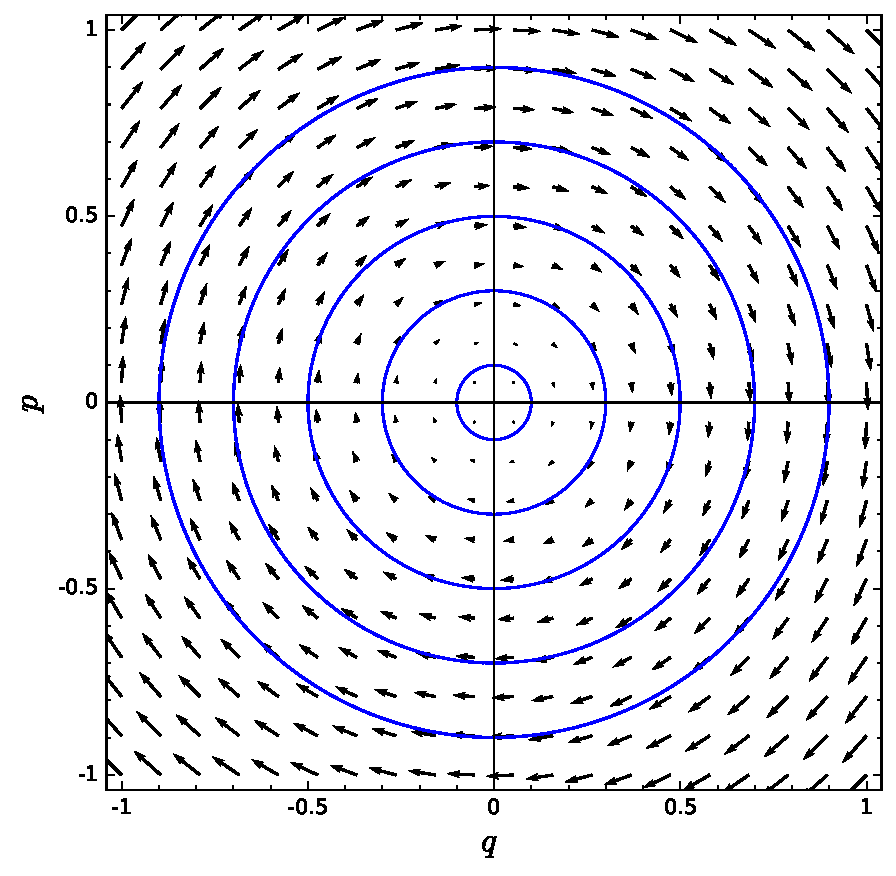
\includegraphics[width=0.4\textwidth]{pics/oscilador}
    \label{fig:oscilador}
    \caption{\small Espacio de fases del oscilador armónico junto al campo y a las curvas de energía constante. En este caso $k=m=1$, de modo que las curvas de energía constante son circunferencias de radio $\sqrt{2E}$.}
  \end{figure}

  Ahora, si tomamos unas coordenadas «polares» $(E,\phi)$, donde $\phi$ es la coordenada angular en cada una de estas elipses, la dinámica del sistema queda mucho más simplificada: 
  \begin{equation*}
    \begin{cases}
    E(t)&=E(0) \\
    \phi(t)&=\phi(0)-\omega t.
  \end{cases}
  \end{equation*}
  Sin embargo, ¿será canónica la transformación $(q,p) \rightarrow (E,\phi)$? Para ello, veamos cómo se comporta la forma $\Omega_1=\dd p\wedge \dd q$ con el cambio
  \begin{equation*}
    \begin{cases}
      q(E,\phi)=\sqrt{\frac{2E}{k}}\cos\phi\\
      p(E,\phi)=\sqrt{2mE}\sin \phi.
    \end{cases}
  \end{equation*}
  Tenemos entonces
  \begin{equation*}
    \begin{cases}
      \dd q= \frac{1}{\sqrt{2kE}}\cos \phi \dd E - \sqrt{\frac{2E}{k}} \sin \phi \dd \phi \\
      \dd p= \sqrt{\frac{m}{2E}}\sin \phi \dd E + \sqrt{2mE} \cos \phi \dd \phi,
    \end{cases}
  \end{equation*}
  y 
  \begin{equation*}
    \Omega_1= \dd p \wedge \dd q = -\sqrt{\tfrac{m}{k}}(\cos^2 \phi + \sin^2 \phi) \dd E \wedge \dd \phi= -\tfrac{1}{\omega} \dd E \wedge \dd \phi.
  \end{equation*}
  Por tanto, si definimos la \emph{variable de acción}, $J=-\frac{E}{\omega}$, entonces $\Omega_1=\dd J \wedge \dd \phi$ y $(J,\phi)$ son unas coordenadas de Darboux.

  Para tratar de dar sentido físico a esta variable $J$, consideremos el área $A_E$ de la región $S_E$ encerrada por la curva de energía constante $M_E$. Por la fórmula del área de la elipse
  \begin{equation*}
    A_E=\pi \sqrt{2mE} \sqrt{\frac{2E}{k}}=2\pi \sqrt{\frac{m}{k}} E= 2 \pi \frac{E}{\omega}= -2\pi J.
  \end{equation*}

  Observemos ahora que como $\Omega_1$ es la forma de área en $\RR^2$, 
  \begin{equation*}
    A_E=\int_{S_E}\Omega_1 = \int_{S_E} \dd p \wedge \dd q = \int_{M_E}p\dd q,
\end{equation*}
donde hemos usado el teorema de Stokes y el hecho de que $\dd p \wedge \dd q= \dd(p\dd q)$. De modo que podemos redefinir la variable de acción en la forma
\begin{equation*}
  J=-\frac{1}{2\pi}\int_{M_E}p \dd q.
\end{equation*}
Este será el aspecto que tengan las variables de acción-ángulo en general para sistemas con un grado de libertad. Regresando ahora a las coordenadas originales, tenemos
\begin{equation*}
  \begin{cases}
    q(J,\phi)=\sqrt{-\frac{2J\omega}{ k}}\cos \phi\\
    p(J,\phi)=\sqrt{-2m\omega J}\sin \phi.
  \end{cases}
\end{equation*}

\paragraph{\bf Oscilador armónico con $n$ grados de libertad}\mbox{}

  Para estudiar un caso de dimensión superior, podemos considerar el sistema formado por $n$ osciladores armónicos no acoplados o, equivalentemente, un oscilador armónico con $n$ grados de libertad. El hamiltoniano del sistema será (tomando $k=m=1$)
  \begin{equation*}
    H(q_1,\dots,q_n,p_1,\dots,p_n)= H_1(q_1,p_1)+ \cdots +H_n(q_n,p_n) = \tfrac{1}{2}\sum_{i=1}^n (p_i^2+q_i^2).
  \end{equation*}
  Este sistema es integrable en el sentido de Liouville. Basta tomar $F=(H,H_2+\cdots+H_{n},H_3+\cdots+H_{n-2},\dots,H_n)$, ya que 
  \begin{equation*}
    \pois{H_i}{H_j} = \sum_{k=1}^n\left( \parcial{H_i}{p_k}\parcial{H_j}{q_k} - \parcial{H_j}{p_k}\parcial{H_i}{q_k}\right)=0
  \end{equation*}
  y las componentes de $F$ son independientes en casi todo punto de $\RR^{2n}$. 
  
  Ahora, dado $a=(a_1,\dots,a_n)\in \RR^n$, $M_a=F^{-1}(a)$ vendrá dado por 
  \begin{equation*}
    \left\lbrace
    \begin{array}{l}
      \tfrac{1}{2}(p_1^2+q_1^2)=a_1-a_2 \\
      \tfrac{1}{2}(p_2^2+q_2^2)=a_2-a_3 \\
\vdots \\
\tfrac{1}{2}(p_n^2+q_n^2)=a_n, 
    \end{array}
    \right.
  \end{equation*}
  que son las ecuaciones de un toro $n$-dimensional. Cada una de las ecuaciones $\frac{1}{2}(p_i^2+q_i^2)=a_i-a_{i+1}$ da una circunferencia $C_{a,i}$ de radio $r_i=\sqrt{2(a_i-a_{i+1}}$, de modo que $M_a=C_{a,1}\times\dots\times C_{a,n}$. Nótese que en este caso los valores críticos son precisamente aquellos $a$ con varias componentes iguales, de forma que los puntos críticos formarán toros de dimensión menor.

  Consideremos $\gamma_{a,i}$ lazos en cada circunferencia $C_{a,i}$, de manera que los $\gamma_{a,i}$ son generadores del grupo fundamental de $M_a$. Entonces podemos definir las variables de acción 
  \begin{equation*}
    J_i(a) = \frac{1}{2\pi}\int_{\gamma_{a,i}} \sum_{k=1}^n p_k \dd q_k.
  \end{equation*}
  La definición de estas variables no depende de la base elegida ya que, por el teorema de Stokes,
  \begin{equation*}
    \int_{\gamma_{i,a}} \sum_{k=1}^n p_k \dd q_k- \int_{\gamma_{i,a}'} \sum_{k=1}^n p_k \dd q_k = \int_{\sigma} \omega=0,
  \end{equation*}
  donde $\sigma$ es la región encerrada por las curvas, ya que $\omega|_{M_a}=0$ y en $M_a$ no hay puntos críticos.

  Consideremos ahora las variables angulares $\phi_i$ a lo largo de cada $C_{i,a}$. Podemos tomar entonces las nuevas coordenadas $(J,\phi)$, con
  \begin{equation*}
      J_i(q,p)=J_i(F(q,p))=\frac{1}{2\pi}\int_{\gamma_{F(q,p),i}} \sum_{k=1}^n p_k \dd q_k 
  \end{equation*}
  y $\phi(q,p)$ las variables angulares en el toro $M_{F(q,p)}$.
  Si la carta $(J,\phi)$ es de Darboux, las ecuaciones de Hamilton pueden integrarse por cuadraturas. Esto se debe a que $J=J(a)$, de modo que, por las ecuaciones de Hamilton,
\begin{equation*}
  \parcial{H}{\phi_i}=-\dot{J_i}=0.
\end{equation*}
Por tanto, $H=H(J_1(a),\dots,J_n(a))$ y 
\begin{equation*}
  \dot{\phi_i}=\parcial{H}{J_i} = \omega_j(a),
\end{equation*}
con $\omega_j$ constante en $M_a$. Las ecuaciones de Hamilton quedan entonces integradas en la forma
\begin{equation*}
  \begin{cases}
  J(t)= & J(a) \\
  \phi(t) = & \phi(0) + \omega(a) t.
\end{cases}
\end{equation*}


\section{Movimiento condicionalmente periódico}\label{sec:promedios}
Una vez tenemos a nuestra disposición el teorema de Arnold-Liouville, sabemos que el flujo en los toros invariantes de los sistemas integrables en el sentido de Liouville será muy sencillo. En esta sección vamos a estudiar el flujo en estos toros y obtendremos un teorema muy importante sobre este tipo de sistemas.

  En primer lugar, consideremos un $2$-toro invariante con la dinámica del teorema (por ejemplo, el asociado a los niveles de energía de un oscilador armónico bidimensional). Sea $(\theta_1,\theta_2)$ un punto en el toro y su trayectoria bajo el flujo hamiltoniano $\gamma(t)=\varphi_t(\theta_1,\theta_2)=(\theta_1+\omega_1t,\theta_2+\omega_2t)$. Si $\omega_1/\omega_2=m/n$ es racional, entonces 
  \begin{equation*}
    \gamma\left(\frac{2n\pi}{\omega_2}\right) = (\theta_1+2m\pi,\theta_2+2n\pi)=(\theta_1,\theta_2).
  \end{equation*}
  Es decir, a cierto tiempo la trayectoria «se cierra». Estas órbitas se dicen \emph{periódicas}. 
 
  Sin embargo, si $\omega_2/\omega_1$ es irracional, dado un ángulo $\alpha$ y sea $T$ tal que $\alpha=\theta_1+\omega T$, entonces, sea $T_n=T+2n\pi/\omega_1$, $\alpha=\theta_1+\omega_1(T_n)$ para cada $n\in \NN$. Ahora, la aplicación
  \begin{equation*}
    \begin{array}{rcl}
    g:\SF^1 & \longrightarrow &\SF^1 \\
  \phi & \longmapsto & \phi + 2\pi\frac{\omega_2}{\omega_1},
  \end{array}
\end{equation*}
es una rotación de ángulo un múltiplo irracional de $2\pi$ en la circunferencia del toro de ángulo $\alpha$. Entonces, como ya vimos por el teorema de recurrencia de Poincaré, $\{g^n(\phi)|n\in \NN\}$ es denso en $\SF^1$. Como esto es válido para todo $\alpha$ y se cumple 
\begin{equation*}
  \gamma(T_n)=(\alpha,g^n(\theta_2)+\omega_2 T),
\end{equation*}
tenemos que $\{\gamma(t)|t \in \RR \}$ es denso en el toro. Este tipo de órbitas se llaman \emph{cuasiperiódicas}. Una forma sencilla de visualizar esto es mediante las \emph{figuras de Lissajous} 
\begin{equation*}
  L_{\omega}=\{(\cos t, \cos \omega t) | t \in \RR\},
\end{equation*}
ver figura \ref{fig:lissajous}.
\begin{figure}[h!]
  \centering
  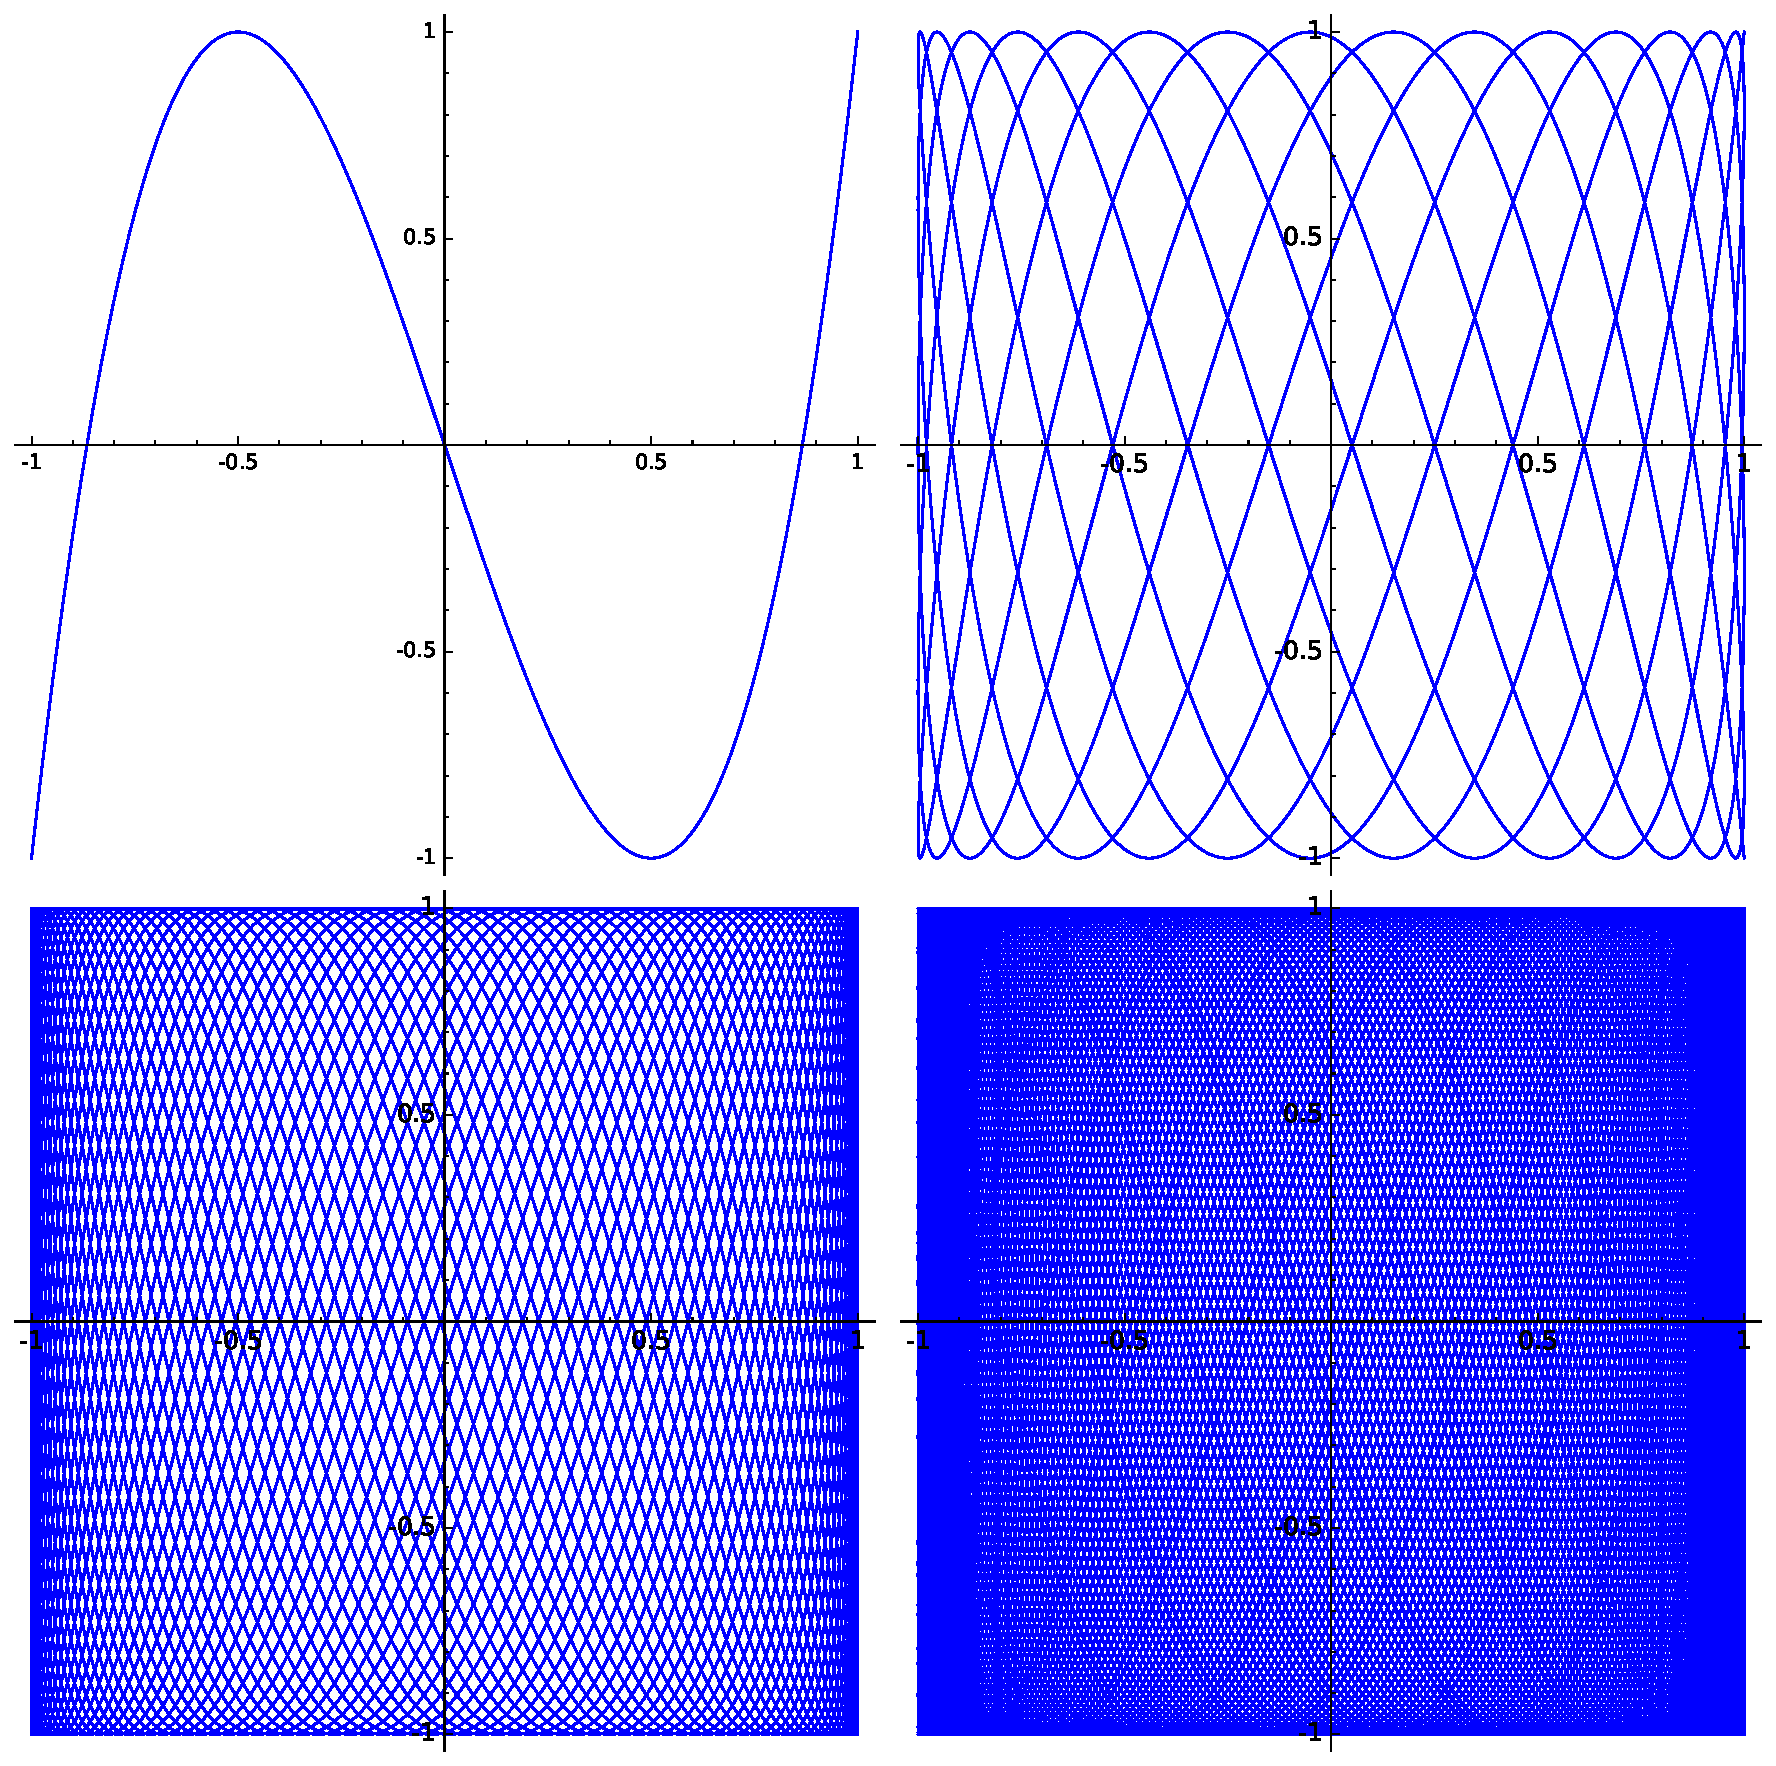
\includegraphics[width=0.6\textwidth]{pics/lissajous}
  \caption{\small Figuras de Lissajous para $\omega=3,$ $3.1,$ $3.14,$  y $3.1416$, $t \in (0,128\pi)$ con pasos de $0.01$.}
  \label{fig:lissajous}
\end{figure}

Vamos a generalizar ahora estas ideas al caso $n$-dimensional.

\begin{defn}[Movimiento condicionalmente periódico en $\TT^n$]
  \em
  Sean $\TT^n$ el toro n-dimensional y $\phi=(\phi_1,\dots,\phi_n)$ coordenadas angulares. Se entiende por un \emph{movimiento condicionalmente periódico} en el toro el flujo uniparamétrico dado por 
  \begin{equation*}
    \phi(t)=\phi(0)+\omega t
  \end{equation*}
  con $\omega=(\omega_1,\dots,\omega_n)$ \emph{frecuencias} constantes en el toro. Las frecuencias $\omega$ se dicen \emph{independientes} si, sea $k \in \ZZ^n$, entonces $\esc{k}{\omega}=0$ si y sólo si $k=0$.
\end{defn}
\begin{defn}[Promedios espacial y temporal]
  \em
  Sea $f:\TT^n \rightarrow \RR$ una función integrable Riemann,
  \begin{enumerate}
    \item El \emph{promedio espacial} de $f$ en $\TT^n$ es el número
      \begin{equation*}
	\bar{f}=\frac{1}{(2\pi)^n}\int_0^{2\pi} \cdots \int_0^{2\pi} f(\phi) d\phi_1,\dots,d\phi_n.
      \end{equation*}
    \item El \emph{promedio temporal} de $f$ en $\TT^n$ es la función
      \begin{equation*}
	f^*(\phi_0)=\lim_{T\rightarrow \infty} \int_0^{T}f(\phi_0+\omega t) dt,
      \end{equation*}
      definida en los puntos $\phi_0$ en los que exista el límite.
  \end{enumerate}
\end{defn}

\begin{thm}[Teorema de los promedios]
  Si $f:\TT^n \rightarrow \RR$ es una función integrable Riemann y las frecuencias $\omega$ son independientes, el promedio temporal está bien definido en todo el toro $\TT^n$ y coincide en todo punto con el promedio espacial.
\end{thm}
\begin{proof}
    En primer lugar, consideramos funciones de la forma $e^{i\esc{k}{\phi}}$, $k\in \ZZ^n$. Si $k=0$, entonces $\bar{f}=f=f^*=1$. Si $k\neq0$, $\bar{f}$ es una integral a periodos en funciones trigonométricas, luego es igual a 0. Por otra parte
     \begin{equation*}
       \int_0^T e^{i\esc{k}{\phi_0 + \omega t}} dt= e^{i\esc{k}{\phi_0}}\int_0^T e^{i\esc{k}{\omega}t}dt=e^{i\esc{k}{\phi_0}}\frac{e^{i\esc{k}{\omega}T}-1}{i \esc{k}{\omega}}.
     \end{equation*}
     Por tanto, el promedio temporal será
     \begin{equation*}
       \lim_{T\rightarrow \infty}\frac{e^{i\esc{k}{\phi_0}}}{i \esc{k}{\omega}}\frac{e^{i\esc{k}{\omega}T}-1}{T}=0.
     \end{equation*}
     
    Como los promedios dependen linealmente de $f$, también coincidirán para los polinomios trigonométricos
     \begin{equation*}
       f=\sum_{|k|<N}f_ke^{i\esc{k}{\omega}}.
     \end{equation*}

    Dado $\varepsilon >0$, si $f$ es continua y real por el teorema de Weierstrass podemos aproximarla por un polinomio trigonométrico $P$ que cumpla $|f-P|<\frac{1}{2}\varepsilon$. Sean $P_1=P-\frac{1}{2}\varepsilon$, $P_2=P+\frac{1}{2}\varepsilon$ entonces
     \begin{equation*}
       \bar{P_2}-\bar{P_1}=\frac{1}{(2\pi)^n}\int_{\TT^n} (P_2 - P_1) d\phi = \frac{1}{(2\pi)^n}\varepsilon (2\pi)^n= \varepsilon.
     \end{equation*}

    Dado $\varepsilon >0$, si $f$ es real e integrable Riemann, entonces existen dos funciones continuas $f_1,f_2$ tales que $f_1<f<f_2$ y $\int_{\TT^n}\frac{1}{(2\pi)^n}(f_2-f_1)d\phi<\frac{1}{3}\varepsilon$. Tomando ahora $P_1,P_2$ polinomios trigonométricos tales que $P_1<f_1<f_2<P_2$ y $\int_{\TT^n}\frac{1}{(2\pi)^n}(P_i-f_i)d\phi < \frac{1}{3}\varepsilon$, para $i=1,2$, entonces
     \begin{equation*}
       \bar{P_2}-\bar{P_1}=\frac{1}{(2\pi)^n}\int_{\TT^n} (P_2 - P_1) d\phi = \frac{1}{(2\pi)^n}\varepsilon (2\pi)^n= \varepsilon.
     \end{equation*}

    Por último, sea $\varepsilon>0$, entonces existen dos polinomios trigonométricos $P_1,P_2$ tales que $P_1<f<P_2$ y $\bar{P_2}-\bar{P_1}<\varepsilon$. Ahora, como $f<P_2$,
     \begin{equation*}
       \frac{1}{T}\int_0^T f(\phi(t))dt < \frac{1}{T}\int_0^T P_2(\phi(t))dt,
     \end{equation*}
     luego
     \begin{equation*}
       \left| \frac{1}{T}\int_0^T f(\phi(t))dt- \bar{f} \right| <\left| \frac{1}{T}\int_0^T P_2(\phi(t))dt- \bar{f} \right| < \left| \frac{1}{T}\int_0^T P_2(\phi(t))dt- \bar{P_2}\right| + |\bar{P_2}-\bar{f}|.
     \end{equation*}
     Pero, como $P_1<f<P_2$, por la monotonía de la integral $\bar{P_1}<f<\bar{P_2}$, luego $|\bar{P_2}-\bar{f}|<|\bar{P_2}-\bar{P_1}|<\varepsilon$. Además, como $P_2$ es un polinomio trigonométrico existe un $T_0$ tal que, si $T>T_0$
     \begin{equation*}
       \left| \frac{1}{T}\int_0^T P_2(\phi(t))dt- \bar{P_2}\right| < \varepsilon .
     \end{equation*}
     Finalmente, obtenemos lo que queríamos probar
     \begin{equation*}
       \left| \frac{1}{T}\int_0^T f(\phi(t))dt- \bar{f} \right| <\left| \frac{1}{T}\int_0^T P_2(\phi(t))dt- \bar{P_2}\right| + |\bar{P_2}-\bar{f}|<\varepsilon + \varepsilon = 2\varepsilon,
     \end{equation*}
     luego $f^*(\phi_0)=\lim_{t\rightarrow \infty}\frac{1}{T}\int_0^T f(\phi(t)) dt = \bar{f}$.
\end{proof}
\begin{corol}
  Si las frecuencias son independientes, entonces, para todo $\phi_0 \in \TT^n$, \[\{\phi(t)=\phi_0+\omega t|t\in \RR\}\] es denso en el toro $\TT^n$.
\end{corol}
\begin{proof}
  En caso contrario, podemos tomar un abierto $D$ del toro que no tiene ningún punto de la trayectoria $\phi(t)$. Construimos la función 
  \begin{equation*}
    f(\phi)=\left\lbrace
    \begin{array}{ll}
      0 & \text{si } \phi \not\in D \\
      \frac{(2\pi)^n}{\int_D d\phi} & \text{si } \phi \in D.
    \end{array}
    \right.
  \end{equation*}
  Claramente, $\bar{f}=1$, pero $f^*(\phi_0)=0$, lo que contradice el teorema de los promedios.
\end{proof}
\begin{corol}
  Sea $D\subset \TT^n$ un conjunto medible Jordan. Sea $A_D=\{t\in \RR | \phi(t) \in D\}$ (que también es medible Jordan) y sea $\tau_D(T)=\int_0^T\chi_{A_D}(t)dt$. Entonces
  \begin{equation*}
    \lim_{T\rightarrow \infty}\frac{\tau_D(T)}{T}= \frac{\mathrm{Vol}(D)}{(2\pi)^n}.
  \end{equation*}
\end{corol}
\begin{proof}
  Aplicamos el teorema a $\chi_D$, entonces $\int_0^T \chi_D(\phi(t))dt=\int_0^T \chi_{A_D}(t)dt=\tau_D(t)$ y $\bar{\chi}_D=(2\pi)^{-n}\mathrm{Vol}(D)$. Finalmente, por el teorema de los promedios
  \begin{equation*}
    \bar{\chi}_D=\frac{\mathrm{Vol}(D)}{(2\pi)^n}=\lim_{T\rightarrow \infty}\frac{1}{T}\int_0^T \chi_D(\phi(t))dt=\lim_{T\rightarrow \infty}\frac{\tau_D(T)}{T}.
  \end{equation*}
\end{proof}

\section{Sistemas con un grado de libertad}
En esta sección damos algunas generalidades sobre los sistemas hamiltonianos con un grado de libertad que, como ya hemos visto, son todos integrables en el sentido de Liouville. Uno de los ejemplos más característicos es el péndulo simple, que estudiamos a continuación.
  
\paragraph{\bf El péndulo simple}\mbox{}
  
  Consideramos un péndulo de masa $m=1$ cuya «cuerda» es una barra rígida de masa despreciable y longitud $1$. El espacio de configuración del péndulo es entonces la circunferencia unidad $\SF^1$ y su espacio de fases será el fibrado tangente de $\SF^1$, que no es otra cosa que un cilindro. Tomando como coordenada generalizada el ángulo $\phi$ de desviación del péndulo respecto de la vertical, el hamiltoniano viene dado por 
  \begin{equation*}
    H(\phi,p)=\frac{1}{2}p^2 - g\cos\phi,
  \end{equation*}
  donde $g$ es la aceleración de la gravedad y hemos tomado el centro como origen de energía potencial.
  \begin{figure}[h]
    \centering
    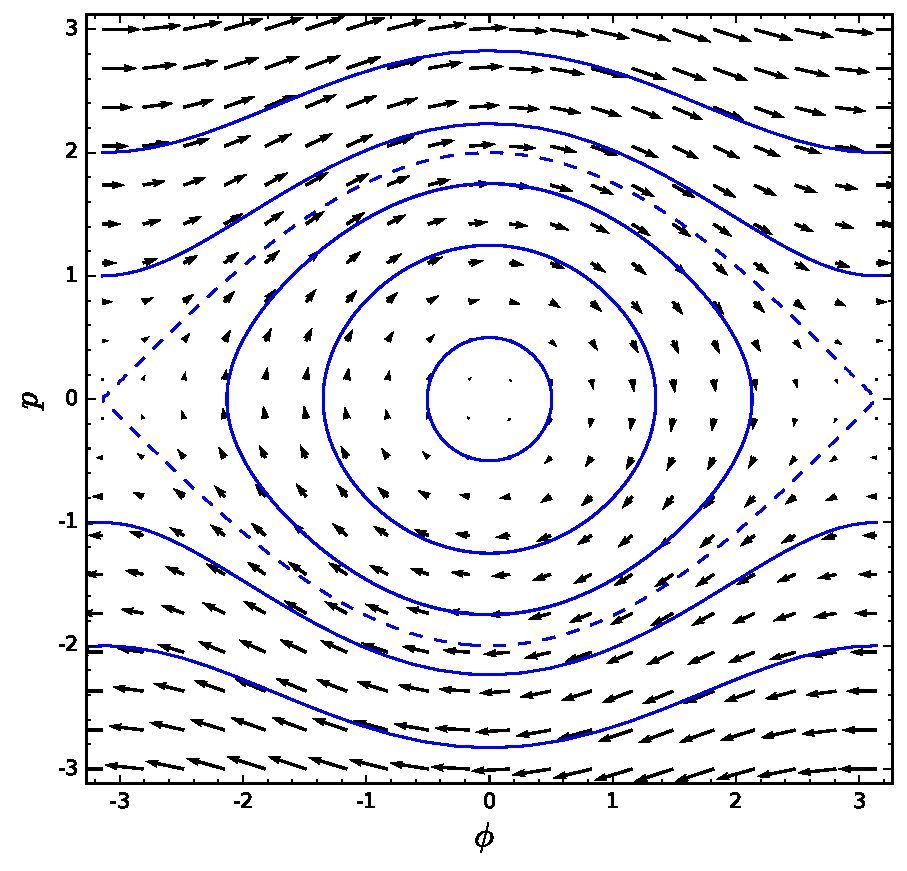
\includegraphics[width=0.4\textwidth]{pics/pendulo}
    \label{fig:pendulo}
    \caption{\small Espacio de fases del péndulo junto al campo hamiltoniano y las curvas de nivel. Nótese que el lado derecho ($\phi=\pi$) está identificado con el lado izquierdo ($\phi=-\pi$), ya que se trata de un cilindro.}
  \end{figure}
  Como podemos ver en la figura \ref{fig:pendulo}  las trayectorias son cerradas, luego cada curva de energía constante es compacta. Para estudiar los puntos críticos, nótese que $\dd H$ es distinta de 0 en todo punto exceptuando los casos $(\phi=0,p=0)$ y $(\phi=\pi,p=0)$, que corresponden a puntos de equilibrio (el primero, estable, el segundo, inestable) donde la trayectoria es sólo un punto. La curva que aparece punteada en la figura, de ecuación
  \begin{equation*}
    g=H(\phi,p)=\frac{1}{2}p^2 - g \cos\phi ,
  \end{equation*}
   corresponde al punto de equilibrio y a dos trayectorias que tienden asintóticamente al punto de equilibrio inestable. Este conjunto no es un toro de Liouville ya que contiene al punto crítico $(\pi,0)$. Estas trayectorias son matemáticamente factibles aunque su realización práctica parezca una tarea imposible. Las curvas que quedan dentro de la curva punteada corresponden a movimientos de oscilación en torno al punto de equilibrio estable, mientras que las que quedan fuera corresponden a movimientos de rotación del péndulo alrededor de su centro. 

   \paragraph{\bf Puntos críticos de los sistemas con un grado de libertad}\mbox{}

   Los dos tipos de punto crítico que presenta el péndulo simple se conocen como \emph{centros}, para el $(0,0)$ y \emph{sillas}, para el $(\pi,0)$. Podemos probar que, de hecho esos son los únicos tipos de punto crítico que puede presentar un sistema hamiltoniano en $\RR^2$. En efecto, supongamos que $(0,0)$ es un punto de equilibrio de un sistema hamiltoniano. Podemos escribir las ecuaciones de Hamilton en la forma
   \begin{equation*}
     \left(
     \begin{array}{c}
       \dot q \\
       \dot p
     \end{array}
     \right)=
\left(
     \begin{array}{cc}
       0 & -1\\
       1 & 0
     \end{array}
     \right)
\left(
     \begin{array}{c}
       \parcial{H}{q} \\
       \parcial{H}{p},
     \end{array}
     \right)
   \end{equation*}
   de modo que su versión linealizada en torno al $(0,0)$ será
   \begin{equation*}
     \left(
     \begin{array}{c}
       \dot q \\
       \dot p
     \end{array}
     \right)=
\left(
     \begin{array}{cc}
       0 & -1\\
       1 & 0
     \end{array}
     \right)
     \left.
\left(
     \begin{array}{cc}
       \frac{\partial^2 H}{\partial q^2} & \frac{\partial^2 H}{\partial p \partial q} \\
       \frac{\partial^2 H}{\partial q \partial p} & \frac{\partial^2 H}{\partial p \partial p} 
     \end{array}
     \right)
     \right|_{(q,p)=(0,0)}
\left(
     \begin{array}{c}
       q \\
       p
     \end{array}
     \right)
     =J_1 B
\left(
     \begin{array}{c}
       q \\
       p
     \end{array}
     \right)
     =A
\left(
     \begin{array}{c}
       q \\
       p
     \end{array}
     \right).
   \end{equation*}
   De la simetría de la matriz de segundas derivadas $B$ y de las propiedades de la matriz $J_1$, tenemos que $A$ ha de cumplir la condición
   \begin{equation*}
     A^{t}J_1+J_1 A=0.
   \end{equation*}
   Las matrices que cumplen esta condición forman el álgebra de Lie $\mathfrak{sp}(2)$ del grupo simpléctico $\mathrm{Sp}(2)$.

   Ahora, se tiene la siguiente proposición.
   \begin{prop}
     Si $\alpha$ es un autovalor de una matriz $A\in \mathfrak{sp}(2)$ con multiplicidad algebraica $k$, entonces $-\alpha$ es también un autovalor de $A$ con la misma multiplicidad. Si $\alpha=0$ entonces su multiplicidad es par.
   \end{prop}
   \begin{proof}
     Los autovalores son los ceros del polinomio característico $P(\alpha)=\det(\alpha I-A)$. Por tanto, basta probar que $\det(\alpha I-A)=\det(\alpha I + A)$. Esto se ve de la siguiente manera,
     \begin{align*}
       P(\alpha)&=\det(\alpha I-A)=\det(-\alpha J_1^2-J_1B)=\det J_1\det(-\alpha J_1 - B)\\
       &=\det(-\alpha J_1-B)^t=\det (\alpha J_1 - B)=\det(\alpha I - J_1^{-1}B)\\
       &=\det(\alpha I + J_1 B)=\det(\alpha I +A).
     \end{align*}
   \end{proof}
   Por tanto, los autovalores de $A$ son imaginarios, opuestos o ambos cero, luego el punto crítico $(0,0)$ solo puede ser un centro (en el caso de autovalores imaginarios) o un punto de silla (en el caso de autovalores reales opuestos). Como consecuencia de esto tenemos que el sistema hamiltoniano no puede tener puntos \emph{asintóticamente estables}, lo que tal vez era de esperar a la vista de la conservación de la energía y del teorema de Liouville: los puntos asintóticamente estables funcionarían como «fuentes» o «sumideros» del área de Liouville.



   \section{Más sistemas integrables}
   Cuando estudiamos sistemas con varios grados de libertad, la integrabilidad requiere de la existencia de cantidades conservadas adicionales. Como ya vimos en el apartado de simetrías y leyes de conservación, una forma útil de encontrar cantidades conservadas es observar las simetrías del sistema, siguiendo el mecanismo de Noether. En esta sección veremos dos ejemplos donde podemos ver directamente esta relación entre las simetrías y la integrabilidad del sistema.

   \paragraph{\bf El péndulo esférico}\mbox{}

   Un péndulo esférico consiste en una partícula (aquí supondremos de masa $m=1$) enganchada por una barra rígida de masa despreciable y de longitud 1 a un punto del espacio y bajo la acción de la gravedad. Es decir, es como un péndulo simple, solo que no está restringido a oscilar en un solo plano, sino que puede moverse libremente, ver figura \ref{fig:espendulo}.
\begin{figure}[h]
  \centering
  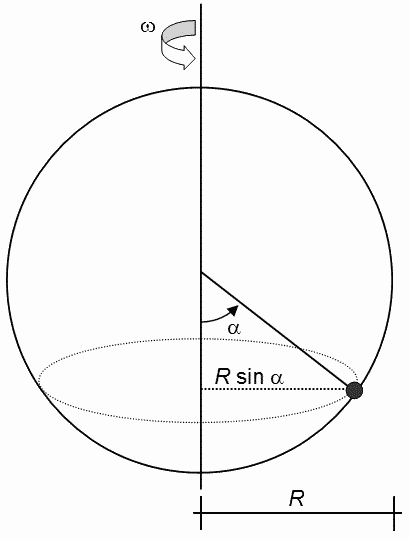
\includegraphics[width=0.3\textwidth]{pics/espendulo.png}
  \caption{\small Péndulo esférico}
  \label{fig:espendulo}
\end{figure}

Podemos considerar el sistema inmerso en $\RR^3$, de modo que el espacio de fases en principio será el espacio simpléctico estándar $6$-dimensional $(\RR^6,\Omega_3)$. Ahora, la ligadura del péndulo restringe el movimiento espacial a una esfera de radio 1, y las velocidades serán siempre tangentes a esta esfera. De este modo, el espacio de fases será
\begin{equation*}
  M=\left\{ (q,p)\in \RR^6 : ||q||=1, \esc{q}{p}=0 \right\},
\end{equation*}
que claramente es difeomorfo al fibrado tangente de la esfera, $T\SF^2$. La forma simpléctica en $M$ será simplemente la restricción de $\Omega_3$ a $M$. El hamiltoniano será la restricción a $M$ de la función 
\begin{align*}
  H :\RR^6&\longrightarrow \RR\\ 
  (q,p) &\longmapsto \tfrac{1}{2m}||p||^2+mgq_3, 
  \end{align*}
  donde $q_3$ es la componente vertical del vector $q=(q_1,q_2,q_3)$.

  Observemos ahora que el sistema es invariante bajo las rotaciones en torno a la vertical. En efecto, si $R\in\mathrm{SO}(3)$ es una rotación en torno a la vertical, como la tercera componente no varía respecto de las rotaciones en torno a la vertical y las rotaciones preservan la norma,
  \begin{equation*}
    H(R(q),R(p))=\tfrac{1}{2m}||R(p)||^2+mgq_3=\tfrac{1}{2m}||p||^2+mgq_3=H(q,p).
  \end{equation*}
  Por tanto, la tercera componente del momento angular $L_3=q_1p_2-q_2p_1$ es una cantidad conservada del sistema $(M,H)$. Como $\dim(M)=4$ y hemos encontrado una cantidad conservada del sistema a parte del propio hamiltoniano, no es difícil comprobar que $H$ y $L_3$ son independientes para casi todo punto, luego el sistema $(M,H)$ será integrable en el sentido de Liouville.

  \paragraph{\bf El potencial central}\mbox{}

  Consideremos el caso genérico de una partícula moviéndose en el espacio sujeta a una fuerza central, es decir, dirigida siempre hacia el origen y cuyo valor dependa solo de la distancia de la partícula a este. Un ejemplo típico sería el de una partícula moviéndose en un potencial kepleriano ($V(r)=-k/r$) (por ejemplo, la Tierra alrededor del Sol) o en un potencial coulombiano (por ejemplo, un electrón que ``gira'' en torno a un núcleo atómico, despreciando toda clase de efectos cuánticos, si es que eso fuera posible). El espacio de fases del sistema es el espacio simpléctico estándar $6$-dimensional $(\RR^6,\Omega_3)$ y el hamiltoniano viene dado por la función
  \begin{equation*}
    H(q,p)=\tfrac{1}{2m}||p||^2+V(||q||).
  \end{equation*}
  Claramente, el sistema es invariante bajo rotaciones ya que, si $R\in \mathrm{SO}(3)$ es una rotación, entonces, como las rotaciones preservan la norma
  \begin{equation*}
    H(R(q),R(p))=\tfrac{1}{2m}||R(p)||^2+V(||R(q)||)=\tfrac{1}{2m}||p||^2+V(||q||)=H(q,p).
  \end{equation*}
  Como consecuencia, se conserva el momento angular $L=q\times p$. En particular, se conservarán $L^2=\esc{L}{L}$ y $L_3=q_1p_2-q_2p_1$. Ahora, si calculamos el corchete de Poisson
  \begin{equation*}
    \pois{L^2}{L_3}=\sum_{i=1}^3\pois{L_i^2}{L_3}=\sum_{i=1}^32L_i\pois{L_i}{L_3},
  \end{equation*}
  por la regla de Leibniz. Ahora, como $\pois{L_3}{L_3}=0$, tenemos 
  \begin{equation*}
    \pois{L^2}{L_3}=2L_1\pois{L_1}{L_3}+2L_2\pois{L_2}{L_3}.
  \end{equation*}
  Basta entonces hallar 
  \begin{equation*}
    \pois{L_1}{L_3}=\pois{q_2p_3-q_3p_2}{q_1p_2-q_2p_1},
  \end{equation*}
  que, usando la linealidad del corchete de Poisson y la identidad de Jacobi y teniendo en cuenta que $\pois{q_i}{q_j}=\pois{p_i}{p_j}=0$ podemos desarrollar hasta llegar a
  \begin{equation*}
    \pois{L_1}{L_3}=-p_3q_1\pois{q_2,p_2}-q_3p_1\pois{p_2}{q_2}=+p_3q_1-q_3p_1=-L_2.
  \end{equation*}
Un cálculo análogo muestra que $\pois{L_2}{L_3}=L_1$, de modo que
\begin{equation*}
  \pois{L^2}{L_3}=-2L_1L_2+2L_2L_1=0.
\end{equation*}

Por tanto, $H$, $L^2$ y $L_3$ son $3$ funciones en involución y además es posible comprobar que son independientes en casi todo punto de $\RR^6$, de modo que el sistema $(M,H)$ es integrable en el sentido de Liouville.

